% !TEX program = xelatex

\documentclass[hidelinks, 12pt, a4paper]{article}

\usepackage{fontspec}
\setmainfont[Ligatures=TeX]{Linux Libertine O}

\usepackage[hidelinks, colorlinks = true, urlcolor = blue]{hyperref}

\usepackage{indentfirst}
\usepackage{graphicx}
\usepackage[left=2cm,right=2cm,top=2.5cm,bottom=2.5cm]{geometry}
\usepackage{lipsum}

%\setlength{\parindent}{1em}
%\setlength{\parskip}{1em}\title{Εργασία Στατιστικής}

%\title{Java socket programming \\ 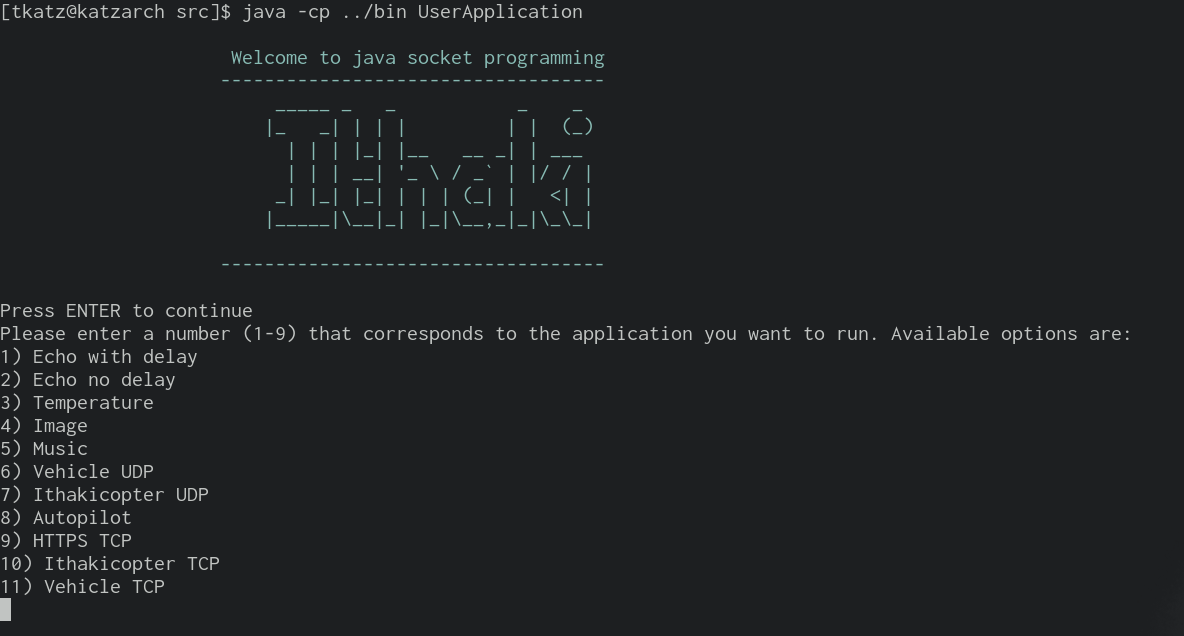
\includegraphics[width=\textwidth]{assets/login.png}}
% \author{Θεόδωρος Κατζάλης \\ ΑΕΜ:9282 \\ katzalis@auth.gr}
% \date{19/07/2020}

\begin{document}

\begin{titlepage}

\begin{figure}[h!]
  \begin{center}
    
\includegraphics[width=3cm]{assets/auth.pdf}
    \label{fig:cover_auth_logo}
  \end{center}
\end{figure}

\centering
\Large Αριστοτέλειο Πανεπιστήμιο Θεσσαλονίκης\\
\Large Πολυτεχνική Σχολή\\
%\large Τμήμα Ηλεκτρολόγων Μηχανικών και Μηχανικών Υπολογιστών\\
%\large Τομέας Τηλεπικοινωνιών

\vspace{\fill}

\LARGE \textbf{Java socket programming} \\
\LARGE \textbf{Δίκτυα 2}

\vspace{\fill}

\Large Θεόδωρος Κατζάλης \\
\Large ΑΕΜ:9282 \\ 
\Large katzalis@auth.gr

\vspace{\fill}
\raggedright

\centering
\vspace{\fill}
\today

\end{titlepage}

%\maketitle


\pagebreak
\tableofcontents
\pagebreak

% \section{Lorem}
% \lipsum


\section{Εισαγωγή}

Η συγκεκριμένη εργασία αποσκοπεί στην εξοικείωση εννοιών σχετικά με τα δίκτυα υπολογιστών τόσο σε θεωρητικό όσο και σε πρακτικό επίπεδο. Το πρώτο εξασφαλίζεται με την μελέτη και παράθεση βιβλιογραφίας σε πρωτόκολλα επικοινωνίας \textbf{TCP} και \textbf{UDP} ενώ το δεύτερο εξασφαλίζεται, χρησιμοποιώντας την γλώσσα προγραματισμού \textbf{java}, με την δημιουργία δικτυακών εφαρμογών συλλογής πληροφοριών σε συνεργασία με τον server του μαθήματος ithaki με IP 155.207.18.208.

\section{Retransmission timeout}

Σε γενικές γραμμές υπάρχει η ανάγκη πρόβλεψης και επαναπροσδιόρισης των παραμέτρων timeout σε ένα σύστημα επικοινωνίας.

Αξίζει να αναφέρουμε κάποια πράγματα για RTO και για time granularity. RFC και τα σχετικά. Υπάρχουν κάποιες διαφορές σχετικά με το notation που χρησιμοποιούνται στις σχέσεις υπολογισμού των εννοιών RTO, sRRT και RTTd. 

Οι πηγές στις οποίες βασιστήκαμε είναι:
\begin{itemize}
    \item \href{https://www.geeksforgeeks.org/tcp-timers/}{geeks for geeks}
    \item \href{https://tools.ietf.org/html/rfc6298}{RFC}
    \item \href{https://www.saminiir.com/lets-code-tcp-ip-stack-5-tcp-retransmission/}{let's code a tcp/ip}
    \item \href{https://stackoverflow.com/questions/16740014/computing-time-on-linux-granularity-and-precision}{time granularity}
\end{itemize}

\section{Session 1}

\section{Section 2}

\section{UDP}
Hello

\section{Audio streaming protocols}

\section{Πηγαίος κώδικας}

\subsection{User Interface}

\begin{figure}[h!]
\centering
	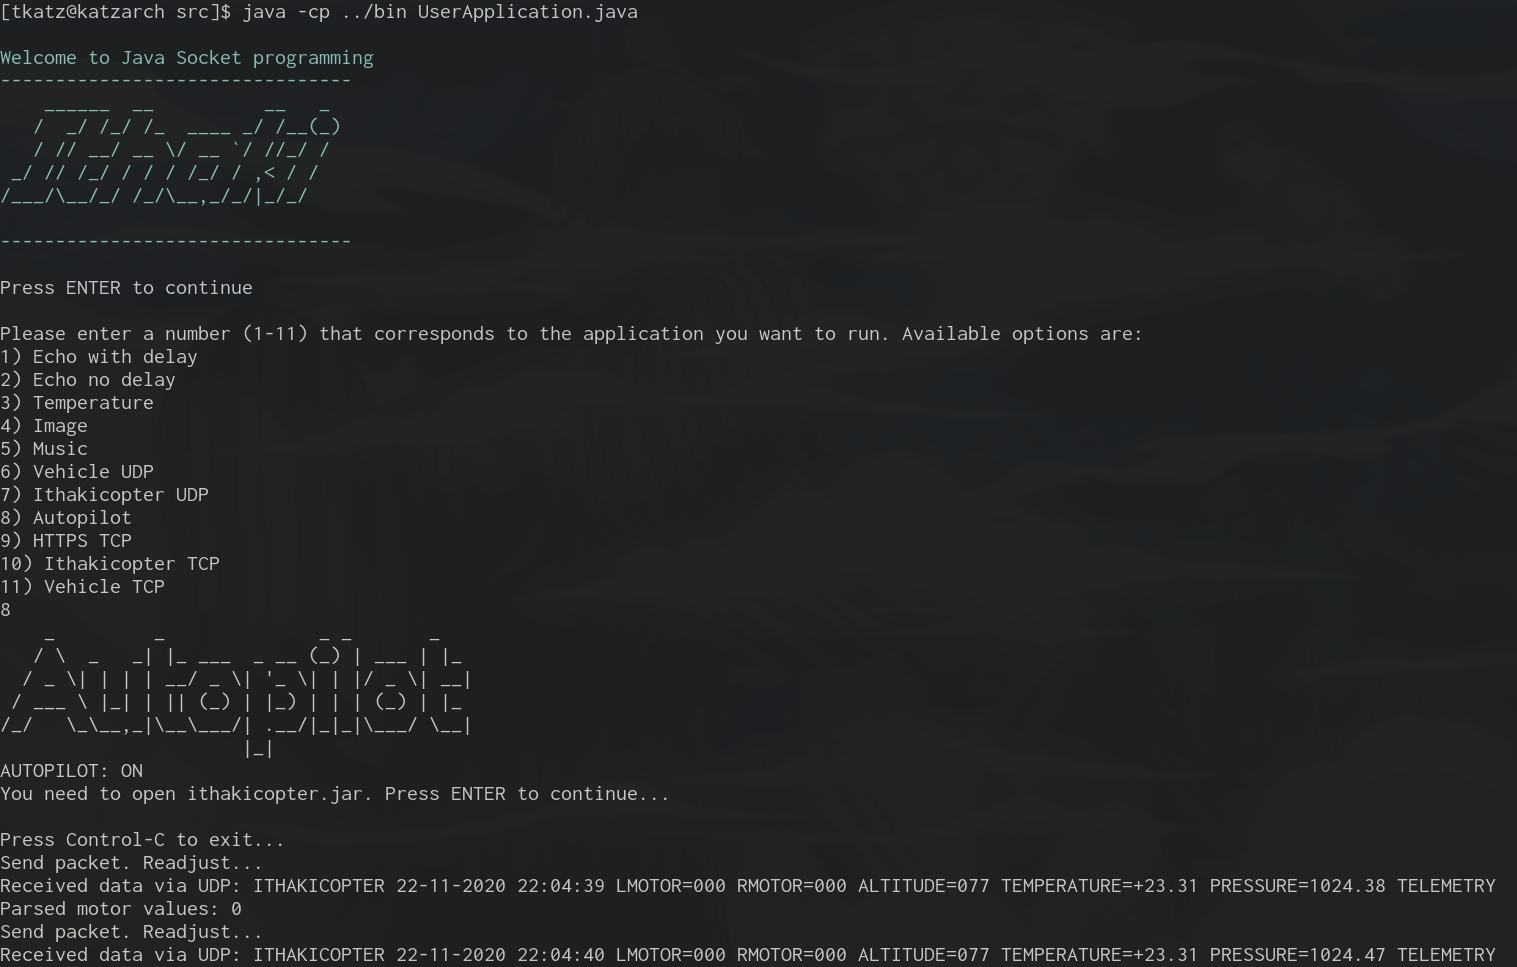
\includegraphics[width=\textwidth]{assets/ui.png}
	\caption{Εκτέλεση προγράμματος σε κέλυφος Bash} 
    \label{fig:ui}
\end{figure}



\section{Statement of originality aka bibliography}
 
\end{document}
